\documentclass[a4paper]{article}

\usepackage[utf8]{inputenc}
\usepackage[portuguese]{babel}
\usepackage{a4wide}
\usepackage[pdftex]{hyperref}
\usepackage{graphicx}
\usepackage{wrapfig}
\usepackage{amsmath}
\usepackage{verbatim}
\usepackage{caption}
\usepackage{subcaption}
\usepackage{float}



\begin{document}

\begin{titlepage}
\begin{center}



\includegraphics[width=0.6\textwidth]{logo.jpg}\\[0.5cm]

{\large Universidade do Minho - Escola de Engenharia}\\[0.5cm]

{\large Relatório do trabalho prático de Sistemas Distribuídos}\\[0.5cm]

% Title
\rule{\linewidth}{0.5mm} \\[0.4cm]
{ \huge \bfseries Matchmaking num jogo online \\[0.4cm] }
\rule{\linewidth}{0.5mm} \\[1.5cm]

% Author and supervisor
\noindent
\begin{minipage}{0.4\textwidth}
  \begin{flushleft} \large
    \emph{Autores :}\\
    Daniel Maia \textsc{(A77531)}\\
    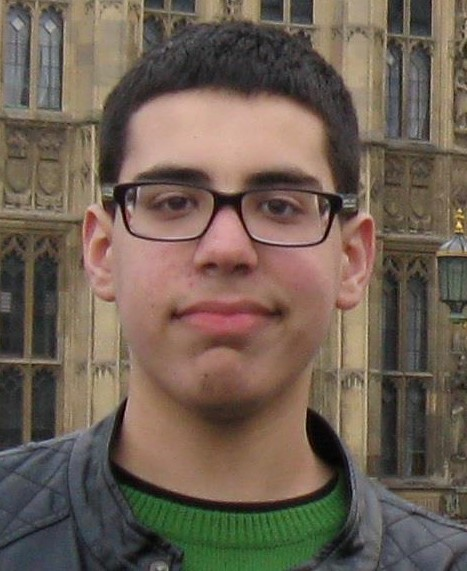
\includegraphics[width=1.5cm]{daniel.jpg}\break
    Diogo Silva\textsc{(A78034)}\\
    
\includegraphics[width=1.5cm]{afonso.jpg}\break
    Marco Silva\textsc{(A79607)}\\
    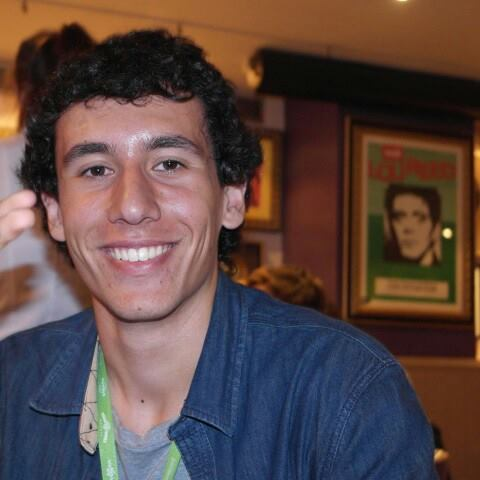
\includegraphics[width=1.5cm]{marco.jpg}\break
  \end{flushleft}
\end{minipage}%
\vfill

% Bottom of the page
{\large Versão 1.0 \\ \today}

\end{center}
\end{titlepage}




\begin{abstract}

\hspace{3mm} 

\end{abstract}

\pagebreak
\tableofcontents

\pagebreak
\section{Introdução}
\label{sec:1}

\hspace{3mm} Neste relatório será apresentado um projeto desenvolvido no âmbito da Unidade Curricular de Sistemas Distribuídos da Universidade do Minho.

\par Este projeto consiste num sistema de gestão de jogadores de um servidor \emph{online} desde o seu registo, autenticação até à disputa do jogo em si. É de salientar que neste projeto no que diz respeito ao jogo em si, é feita apenas uma geração de um resultado aleatório definindo assim a equipa vencedora e a equipa perdedora.



%------------------------------------------------------------------------

\pagebreak
\section{Descrição do problema}
\label{sec:2}

\hspace{3mm} A proposta de trabalho dada para o projeto é o da implementação de uma aplicação distribuída para \textit{matchmaking} num jogo \textit{online}, num estilo semelhante a videojogos tais como Overwatch ou Paladins. Esta aplicação terá a capacidade de, nomeadamente, formar automaticamente duas equipas por partida e permitir a cada jogador um intervalo de tempo para escolher uma personagem, referida como herói, antes da partida iniciar.

\par Cada equipa será constituída por 5 jogadores, cada um com uma classificação pessoal. Esta classificação, determinada pelas vitórias e derrotas sofridas no jogo, terá um valor inteiro entre 0 e 9, e terá no máximo uma diferença unitária entre todos os jogadores de uma dada partida. Tendo encontrado 10 jogadores disponíveis com classificações semelhantes, o servidor dividi-los-á em equipas equilibradas de acordo com as classificações dos mesmos. Para que esta classificação seja guardada, será implementado um sistema de registo e autenticação. Com um nome de utilizador e uma palavra passe, o servidor autentica o jogador sempre que este estabelece ligação ao mesmo.

\par Tendo as duas equipas feitas, os jogadores procederão à fase da escolha dos heróis, dos quais existem 30. Cada jogador poderá escolher qualquer um, desde que este não tenha ainda sido selecionado por outro jogador da mesma equipa. Como tal, cada jogador poderá ver as escolhas de heróis dos elementos da mesma equipa. Qualquer jogador poderá selecionar um herói diferente, caso mude de ideias. Após 30 segundos, a fase de escolha será dada como terminada. Se algum jogador da partida não tiver escolhido um herói, a partida é abortada e cada jogador terá de selecionar a opção de jogar uma vez mais. Caso contrário, será mostrada a composição de ambas equipas a todos os jogadores da partida, nomeadamente o nome de utilizador de cada jogador e respetivo herói. É depois simulada uma partida, cujo resultado aleatório será utilizado para atualizar a classificação de cada jogador, subindo com cada vitória e descendo com cada derrota.

\par Para aceder ao servidor, cada jogador terá acesso a um programa Cliente, com o qual acederá a um Servidor \textit{multithreaded} através de \textit{sockets} TCP. Em concordância com a proposta do trabalho, o protocolo entre os dois será baseado em texto, orientado à linha, e cada \textit{thread} do Servidor escreverá em um e só um \textit{socket}.


\pagebreak
\clearpage
%--------------------------------------------------------------------------

\section{Conceção da Solução}
\label{sec:3}

\subsection{Registo e login}
\label{sec:3.1}
\hspace{3mm} 



\subsection{Matchmaking}
\label{sec:3.2}

\hspace{3mm} O \textit{Matchmaking} consiste na seleção dos jogadores que indicaram que pretendiam jogar seguindo algumas das regras que foram impostas na descrição do projeto como por exemplo a impossibilidade de numa sala de jogo existirem diferenças superiores a 1 unidade no que toca aos níveis dos jogadores intervenientes.

\par Este sistema de \textit{matchmaking} para que a seleção dos jogadores seja feita da forma mais eficiente possível define zonas de agrupação de jogadores para cada um dos níveis possíveis exceto o nível 9. Assim, cada um dos jogadores pode entrar numa sala com o índice do seu nível ou na sala com índice imediatamente abaixo do seu nível. Nos casos de jogadores com nível 0 e 9, estes entram sempre em sala com índice 0 e 8 respetivamente. Finalmente, a decisão entre as ´duas salas possíveis é feita com base na ocupação de cada uma das salas, dando sempre a prioridade à sala que se encontra mais perto de estar completa, ou seja, com mais jogadores.

\par Quando o número de jogadores necessários para passar à proxima fase é atingido (10), todos os jogadores passam à fase seguinte (construção das equipas).


\subsection{Fazer equipas}
\label{sec:3.3}

\hspace{3mm} Para que o jogo seja o mais justo possível, foi desenvolvido um algoritmo para a construção das equipas que tem por base os níveis dos jogadores construido assim duas equipas com o nível médio dos níveis dos jogadores o mais próximo possível.

\par O algoritmo verifica numa primeira fase se o número de jogadores em cada uma das equipas é o mesmo e se se verificar, caso o nível do jogador seja o maior da sala, então o jogador é inserido na equipa que tem um menor número de jogadores com o nível máximo da sala. Ainda com o mesmo número de jogadores em cada uma das equipas mas o jogador tem o menor nível possível na sala, então este é inserido na equipa que tem mais jogadores com o nível máximo na sala. Finalmente, no caso em que o número de jogadores em cada uma das equipas é desigual, então o jogador é inserido na equipa com o menor número de jogadores independentemente do seu nível.

\subsection{Escolha de heróis}
\label{sec:3.4}
\hspace{3mm} 

\subsection{Cálculo dos resultados}
\label{sec:3.5}
\hspace{3mm} 

\pagebreak

%--------------------------------------------------------------------------

\section{Conclusões}
\label{sec:4}

\hspace{3mm} 



\end{document}
